\documentclass[12pt,a4paper]{article}
\usepackage[utf8]{inputenc}

\usepackage{mathtools}
\usepackage{amsmath}
\usepackage{amssymb}
\usepackage{amsthm}
\usepackage{amssymb}
\usepackage{mathdots}
\usepackage[pdftex]{graphicx}
\usepackage{fancyhdr}
\usepackage[margin=1in]{geometry}
\usepackage{multicol}
\usepackage{bm}
\usepackage{listings}
\usepackage{xcolor}
\usepackage{pdfpages}
\usepackage{algpseudocode}
\usepackage{tikz}
\usepackage{enumitem}
\usepackage[T1]{fontenc}
\usepackage{inconsolata}
\usepackage{framed}
\usepackage{wasysym}
\usepackage[thinlines]{easytable}
\usepackage{hyperref}
\usepackage{minted}
\usemintedstyle{perldoc}
\hypersetup{
    colorlinks=true,
    linkcolor=blue,
    filecolor=magenta,      
    urlcolor=blue,
}
\definecolor{codegreen}{rgb}{0,0.6,0}
\definecolor{codegray}{rgb}{0.5,0.5,0.5}
\definecolor{codepurple}{rgb}{0.58,0,0.82}
\definecolor{backcolour}{rgb}{0.95,0.95,0.92}
\lstdefinestyle{mystyle}{
    backgroundcolor=\color{backcolour},   
    commentstyle=\color{codegreen},
    keywordstyle=\color{magenta},
    numberstyle=\tiny\color{codegray},
    stringstyle=\color{codepurple},
    basicstyle=\ttfamily,
    breakatwhitespace=false,         
    breaklines=true,                 
    captionpos=b,                    
    keepspaces=true,                 
    numbers=left,                    
    numbersep=5pt,                  
    showspaces=false,                
    showstringspaces=false,
    showtabs=false,                  
    tabsize=4
}
\lstset{style=mystyle}
\newcommand\numberthis{\addtocounter{equation}{1}\tag{\theequation}}
\newcommand{\rightqed}{
\begin{flushright}
$\blacksquare$
\end{flushright}
}
\newcommand{\solution}{\noindent\textbf{Solution:}\\\indent}
\usepackage{graphics}
\usepackage{subfig}
\graphicspath{ {./images/} }

\title{Eigenvalues and eigenvectors of example graphs}
\author{Kushajveer Singh}
\date{}

\begin{document}
\maketitle

\subsection*{Problem 1}
\textit{
    Prove $\vec{x}=\delta(a) - \delta(b)$ is an eigenvalue of $L_G$ with eigenvector 1.
}

\solution
We need to prove $$L_G\vec{x} = 1\cdot \vec{x}$$

Now,
\begin{align*}
    L_G\vec{x} &= (D_G - M_G)\vec{x} \\
               &= D_G\vec{x} - M_G\vec{x} \numberthis 
\end{align*}

Computing $D_G\vec{x}$. $D_G$ has value = 1 at index $aa$ and $bb$ and 0 at all non-diagonal entries. So multiplying it by $\vec{x}$ would give us
\begin{align}
    D_G\vec{x} &= \begin{cases}
                  0 & i \neq {a,b} \\
                  1 & i = a \\
                  -1 & i = b \\
                  \end{cases} \\ 
               &= \vec{x}
\end{align}

Computing $M_G\vec{x}$. For the column and row at index $a$ and $b$, we have the following values
\begin{equation}
    \begin{cases}
    0 & i \neq c \\
    1 & i = c \\
    \end{cases}
\end{equation}

Therefore, the product $M_G\vec{x} = \vec{0}$ as at all indices $\neq c$, we are doing multiplication by 0 and at index $= c$, we get $1 + (- 1) = 0$ (for product at index $a$, $b$).

Therefore,
\begin{align*}
    L_G\vec{x} &= D_G\vec{x} - M_G\vec{x} \\
               &= \vec{x} - \vec{0} \\
               &= 1\cdot \vec{x} \numberthis
\end{align*}
\rightqed

\newpage
\subsection*{Problem 2(1)}
\textit{
    Prove that $\vec{x}$ has eigenvalue $v$
}

\solution
\begin{align*}
    \langle \vec{x}, \vec{x} \rangle &= (v-1)^2 + v - 1 \\
                                     &= v(v-1)
\end{align*}
and,
\begin{align*}
    L_S\vec{x} &= D_S\vec{x} - M_S\vec{x} \\
               &= \begin{bmatrix}
                  v-1 & 0 & \hdots & 0\\
                  0   & 1 &        & \\
                  \vdots & & \ddots &  \\
                  0      & & & 1 \\ 
                  \end{bmatrix}\begin{bmatrix}
                  -(v-1) \\
                  1 \\
                  \vdots \\
                  1 \\
                  \end{bmatrix} - \begin{bmatrix}
                  0 & 1 & \hdots & 1 \\
                  1 & 0 & \hdots & 0 \\
                  \vdots & \vdots & \ddots & \\
                  1 & 0 & & 0 \\
                  \end{bmatrix}\begin{bmatrix}
                  -(v-1) \\
                  1 \\
                  \vdots \\
                  1 \\
                  \end{bmatrix} \\
              &= \begin{bmatrix}
                  -(v-1)^2 \\
                  1 \\
                  \vdots \\
                  1 \\
                  \end{bmatrix} - \begin{bmatrix}
                  v-1 \\
                  -(v-1) \\
                  \vdots \\
                  -(v-1)  \\
                  \end{bmatrix} \\
              &= \begin{bmatrix}
                  -v(v-1) \\
                  v \\
                  \vdots \\
                  v \\
                  \end{bmatrix}
\end{align*}

If we compare $L_S\vec{x}$ with $\lambda\vec{x}$, we get the eigenvalue equal to $v$.

Computing the Rayleigh quotient,
\begin{align*}
    \frac{\langle \vec{x}, L_S\vec{x} \rangle}{\langle \vec{x}, \vec{x} \rangle} &= \frac{\begin{bmatrix}
                  -(v-1) \\
                  1 \\
                  \vdots \\
                  1 \\
                  \end{bmatrix}^T\begin{bmatrix}
                  -v(v-1) \\
                  v \\
                  \vdots \\
                  v \\
                  \end{bmatrix}}{
                  \begin{bmatrix}
                  -(v-1) \\
                  1 \\
                  \vdots \\
                  1 \\
                  \end{bmatrix}^T\begin{bmatrix}
                  -(v-1) \\
                  1 \\
                  \vdots \\
                  1 \\
                  \end{bmatrix}} \\
            &= \frac{v^2(v-1)}{v(v-1)} \\
            &= v
\end{align*}
\rightqed

\newpage
\subsection*{Problem 2(2)}
\textit{
    Show directly both the $\vec{x}$ is an eigenvector with eigenvalue $v$.
}

\solution
$v$ is only connected to $node 1$.
\begin{align*}
    L_S(\vec{x})(v) &= \vec{x}(v) - \vec{x}(1) \\
                    &= 1 - (-(v-1)) \\
                    &= v
\end{align*}

Therefore, $\vec{x}$ is an eigenvector with eigenvalue $v$.

\subsection*{Problem 3}
\textit{
    Prove graph product of the path graphs.
}

\solution
\begin{figure}[H]
    \centering
    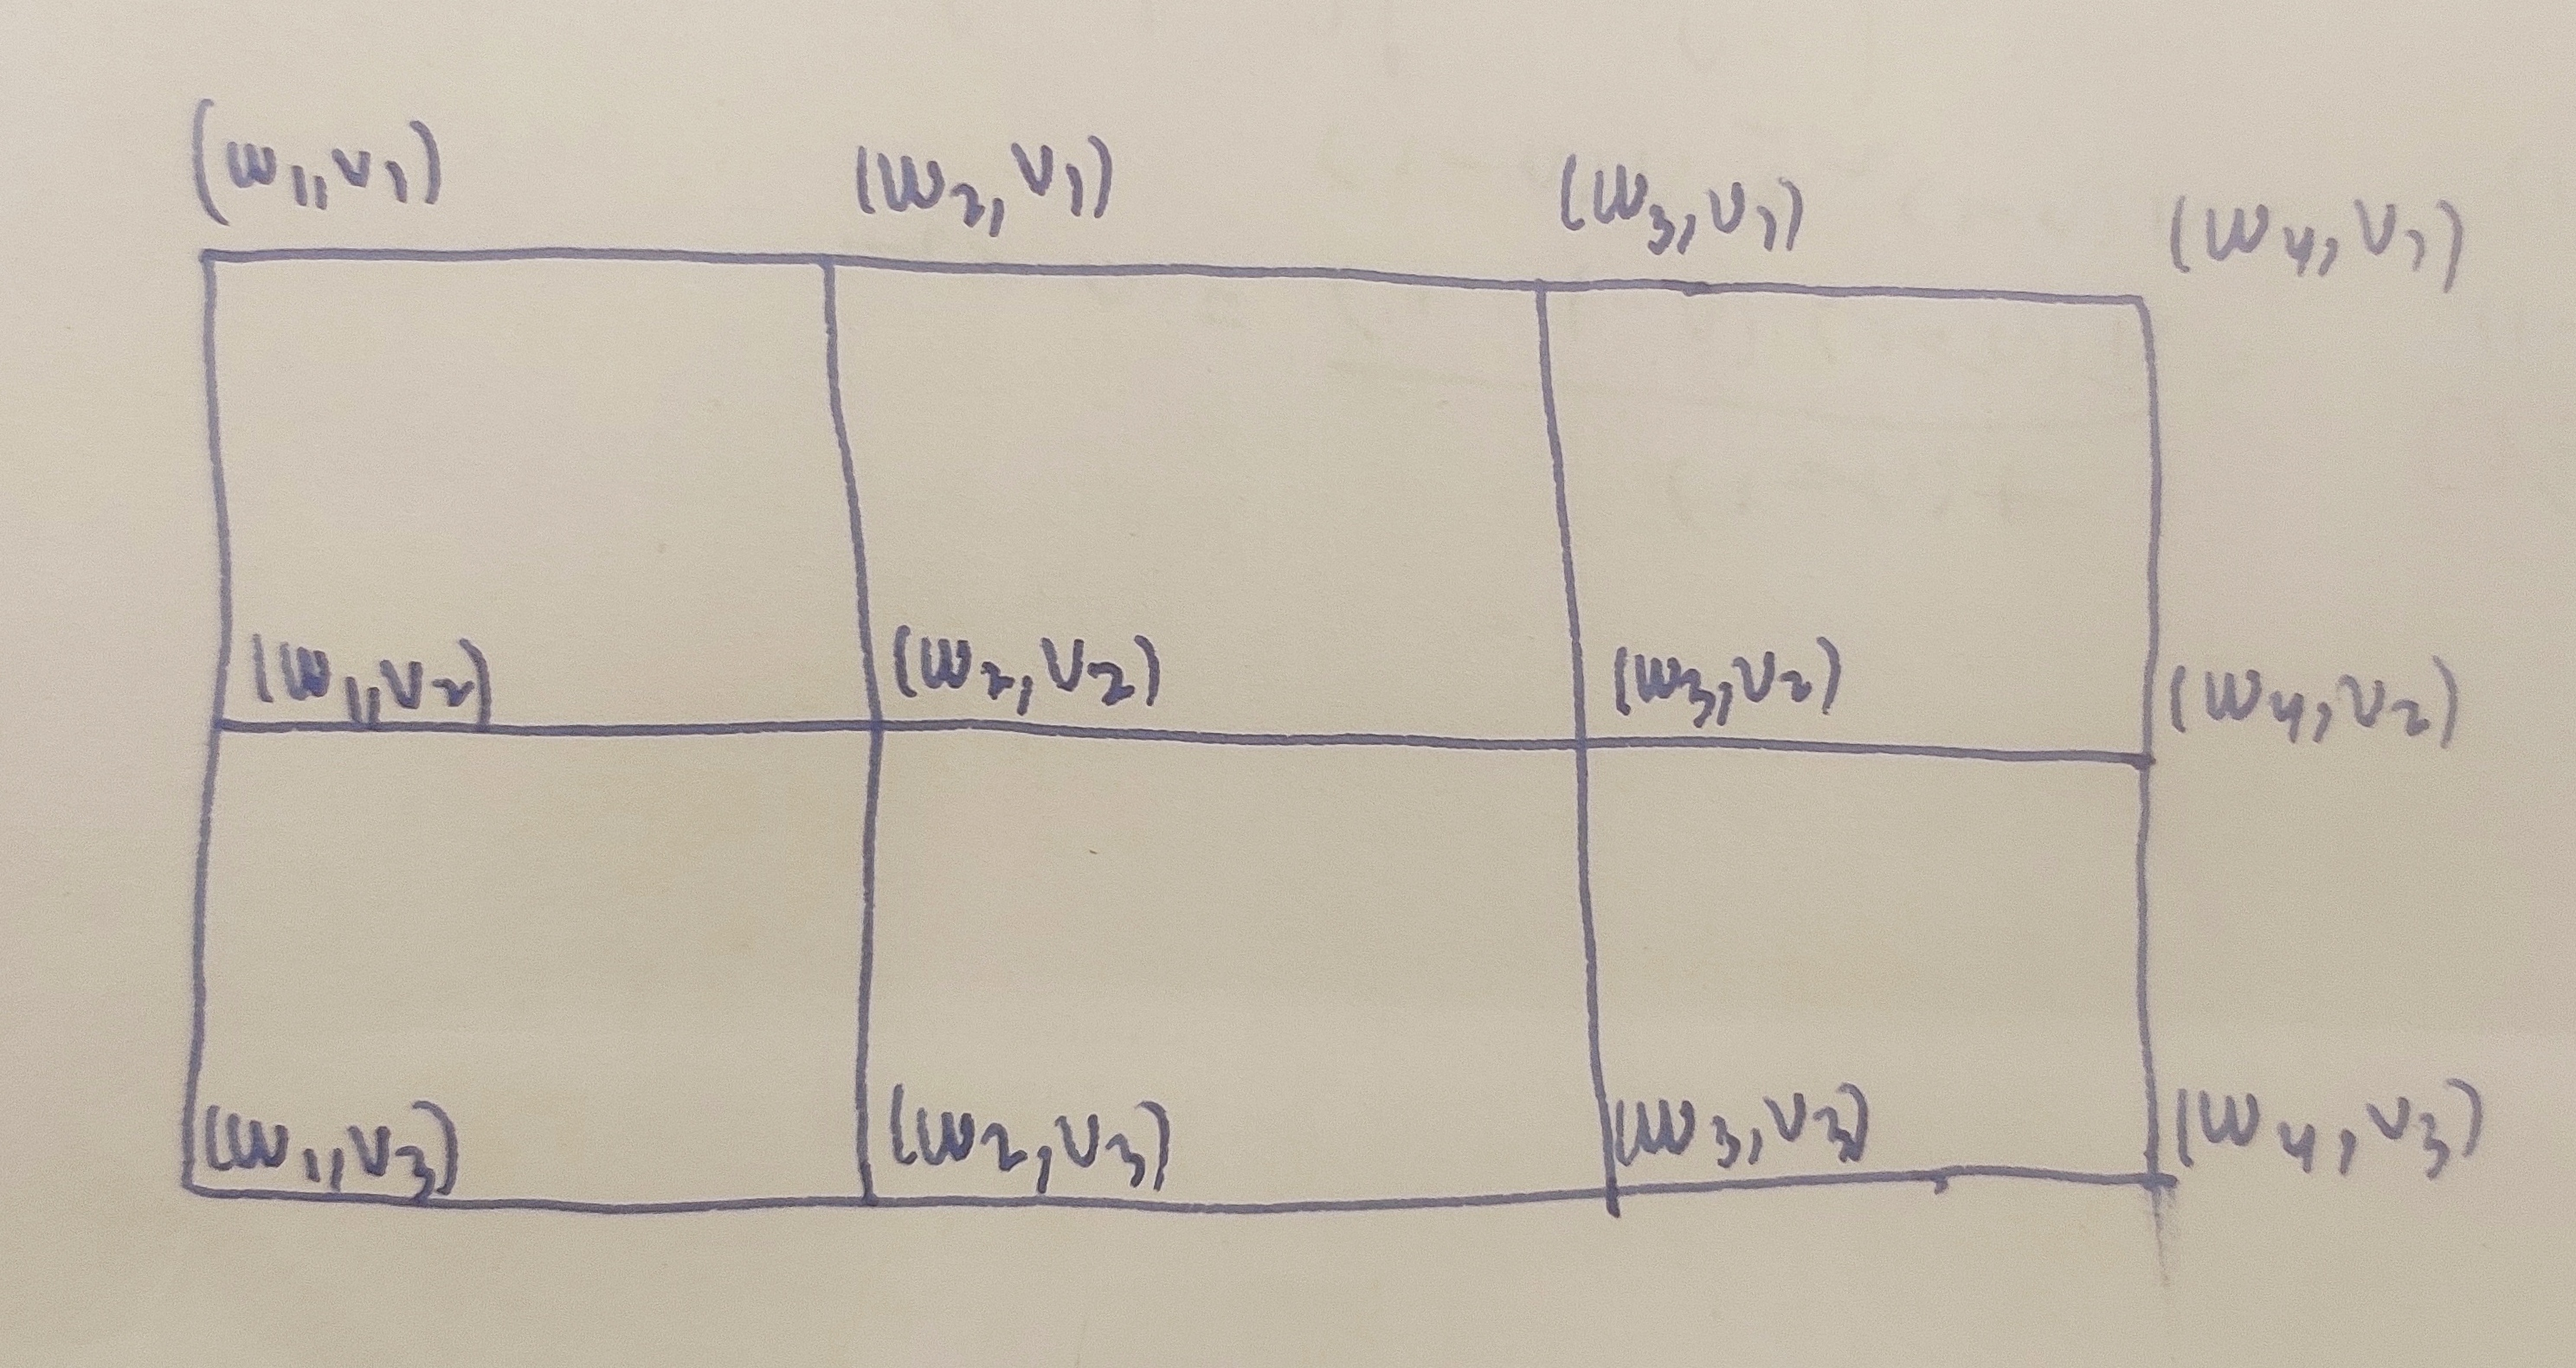
\includegraphics[width=12cm]{01.jpg}
\end{figure}

\newpage
\subsection*{Problem 4}
\textit{
    Show directly both the $\vec{x}$ is an eigenvector with eigenvalue $v$.
}

\solution

Proceeding the proof by induction.

\textbf{Base Case}: $V_{H_1} = \{0,1\}$ and $E_{H_1}=\{0-1\}$, which gives $L_{H_1}=\begin{bmatrix}1 & -1 \\ -1 & 1\end{bmatrix}$ with following eigenvalues and eigenvectors
\begin{align*}
    \lambda_1 = 0\ and\ \vec{\psi}_1 = \begin{bmatrix}1& 1\end{bmatrix}^T \\
    \lambda_2 = -2\ and\ \vec{\psi}_2 = \begin{bmatrix}1& -1\end{bmatrix}^T
\end{align*}

Verifying the statement in question,
\begin{align*}
    \vec{\psi}_0(0) &= (-1)^{0\times 0} = 1 \\
    \vec{\psi}_0(1) &= (-1)^{0\times 1} = 1 \\
    \vec{\psi}_1(0) &= (-1)^{1\times 0} = 1 \\
    \vec{\psi}_1(1) &= (-1)^{1\times 1} = -1 
\end{align*}

Therefore, the base base is true.

\textbf{Assumption}: Assume the statement $\vec{\psi}_y(x) = (-1)^{\sum y_ix_i}$ is true for hypercube of dimension $d-1$.

\textbf{Induction}:
We know $\vec{\psi}_{(y_1, \hdots, y_{d-1})}(x) = (-1)^{\sum y_ix_i}$ for $x=(x_1,\hdots, x_{d-1})\in V_{H_{d-1}}$.

Now for $x_d = 0$
\begin{align*}
    \vec{\psi}_{(y_1, \hdots, y_{d})}(x) &= (-1)^{\sum y_ix_i + y_d\times 0} \\
                                         &= (-1)^{\sum y_ix_i}
\end{align*}

So the statement is true for $x_d = 0$.

For $x_d = 1$
\begin{align*}
    \vec{\psi}_{(y_1, \hdots, y_{d})}(x) &= (-1)^{\sum y_ix_i + y_d\times 1} \\
                                         &= (-1)^{\sum y_ix_i + y_d}
\end{align*}

If $y_d$ is even, then adding $y_d$ to $\sum y_ix_i$ does not change the parity. So the statement is true for $y_d =$ even and $x_d = 1$.

If $y_d$ is odd, then adding $y_d$ to $\sum y_ix_i$ would change the sign of the eigenvector. But this can be countered by changing the sign of the eigenvalue. So the statement is true for $y_d = $ odd and $x_d = 1$.

\rightqed

\newpage
\subsection*{Problem 5(1)}
\textit{
    Compute $A\otimes B$
}

\solution

\begin{align}
    A\otimes B &= \begin{bmatrix}
        6 & 12 \\
        7 & 14 \\
        18 & 24 \\
        21 & 28 \\
    \end{bmatrix} \\
    B\otimes A &= \begin{bmatrix}
        6 & 12 \\
        18 & 24 \\
        7 & 14 \\
        21 & 28 \\
    \end{bmatrix} \\
    \implies A\otimes B &\neq B\otimes A
\end{align}

\subsection*{Problem 5(2)}
\textit{
    Prove that the eigenvectors of $A\otimes B$ are in the form $\vec{\alpha_i}\otimes \vec{\beta_j}$ with corresponding eigenvalues $\lambda_i\mu_j$.
}

\solution
Consider two eigenvector of $A\otimes B$, $\vec{\alpha_i}\otimes \vec{\beta_j}$ and $\vec{\alpha_k}\otimes \vec{\beta_l}$. Checking if these two vectors are orthogonal to each other.
\begin{align*}
    (\vec{\alpha_i}\otimes \vec{\beta_j})^T(\vec{\alpha_k}\otimes \vec{\beta_l}) &= (\vec{\alpha}_i^T\otimes \vec{\beta}_j^T)(\vec{\alpha}_k\otimes \vec{\beta}_l) \\
    &= (\vec{\alpha}_i^T\vec{\alpha}_k)\otimes (\vec{\beta}_j^T\otimes \vec{\beta}_l) \\
    &= 0 \text{ (as $\vec{\alpha}_i^T\vec{\alpha}_k = 0$)}
\end{align*}

Therefore, all the eigenvectors of $A\otimes B$ are orthogonal to each other.

If $\vec{\alpha_i}\otimes \vec{\beta_j}$ is an eigenvector of $A\otimes B$, then
\begin{align*}
    (A\otimes B)(\vec{\alpha_i}\otimes \vec{\beta_j}) &= (A\vec{\alpha_i})\otimes (B\vec{\beta_j}) \\
    &= (\lambda_i\vec{\alpha_i}) \otimes (\mu_j\vec{\beta_j}) \\
    &= \lambda_i\mu_j(\vec{\alpha_i}\otimes \vec{\beta_j}) \numberthis
\end{align*}

As every eigenvector $\vec{\alpha_i}\otimes \vec{\beta_j}$ are orthogonal to each other, therefore $A\otimes B$ has eigenvector $\vec{\alpha_i}\otimes \vec{\beta_j}$ with corresponding eigenvalue $\lambda_i\mu_j$.
\rightqed

\newpage
\subsection*{Problem 5(3)}
\textit{
    Prove that the eigenvectors of $A\oplus B$ are in the form $\vec{\alpha_i}\otimes \vec{\beta_j}$ with corresponding eigenvalues $\lambda_i+\mu_j$.
}

\solution
Consider two eigenvector of $A\otimes B$, $\vec{\alpha_i}\otimes \vec{\beta_j}$ and $\vec{\alpha_k}\otimes \vec{\beta_l}$. Checking if these two vectors are orthogonal to each other.
\begin{align*}
    (\vec{\alpha_i}\otimes \vec{\beta_j})^T(\vec{\alpha_k}\otimes \vec{\beta_l}) &= (\vec{\alpha}_i^T\otimes \vec{\beta}_j^T)(\vec{\alpha}_k\otimes \vec{\beta}_l) \\
    &= (\vec{\alpha}_i^T\vec{\alpha}_k)\otimes (\vec{\beta}_j^T\otimes \vec{\beta}_l) \\
    &= 0 \text{ (as $\vec{\alpha}_i^T\vec{\alpha}_k = 0$)}
\end{align*}

Therefore, all the eigenvectors of $A\oplus B$ are orthogonal to each other.

If $\vec{\alpha_i}\otimes \vec{\beta_j}$ is an eigenvector of $A\oplus B$, then
\begin{align*}
    (A\oplus B)(\vec{\alpha}_i\otimes \vec{\beta}_j) &= (A\otimes I_m + I_n\otimes B)(\vec{\alpha}_i\otimes \vec{\beta}_j) \\
    &= (A\otimes I_m)(\vec{\alpha_i}\otimes \vec{\beta_j}) + (I_n\otimes B)(\vec{\alpha}_i\otimes \vec{\beta}_j) \\
    &= (A\vec{\alpha}_i)\otimes(I_m\vec{\beta}_j) + (I_n\vec{\alpha}_i)\otimes(B\vec{\beta}_j) \\
    &= \lambda_i(\vec{\alpha}_i\otimes\vec{\beta}_j) + \mu_j(\vec{\alpha}_i\otimes\vec{\beta}_j) \\
    &= (\lambda_i + \mu_j)(\vec{\alpha}_i\otimes\vec{\beta}_j) \numberthis
\end{align*}

As every eigenvector $\vec{\alpha_i}\otimes \vec{\beta_j}$ are orthogonal to each other, therefore $A\otimes B$ has eigenvector $\vec{\alpha_i}\otimes \vec{\beta_j}$ with corresponding eigenvalue $\lambda_i+\mu_j$.
\rightqed

\subsection*{Problem 5(4)}
\textit{
    Prove $L_{G\times G'} = L_G\oplus L_{G'}$
}

\solution
The basis vectors of $L_G$ and $L_{G'}$ are given as
\begin{align*}
    L_G: \mathbb{R}^{v_G} \rightarrow \mathbb{R}^{v_G} &\implies v_1, \hdots, v_{v_G}\ for\ \mathbb{R}^{v_G} \\
    L_{G'}: \mathbb{R}^{v_{G'}} \rightarrow \mathbb{R}^{v_{G'}} &\implies v_1', \hdots, v_{v_G'}'\ for\ \mathbb{R}^{v_G'}
\end{align*}

The basis vectors of $L_G \oplus L_{G'}$ is
\begin{align}
    L_G\oplus L_{G'}: \mathbb{R}^{v_{G}+v_G'} \rightarrow \mathbb{R}^{v_{G}+v_G'} &\implies v_1\otimes v_1', \hdots, v_{v_G}\otimes v_{v_G}'\ for\ \mathbb{R}^{v_G+v_G'} \label{eq:1}
\end{align}

The basis vectors of $L_{G\times G'}$ is
\begin{align}
    L_{G\times G'}: \mathbb{R}^{v_{G\times G'}} \rightarrow \mathbb{R}^{v_{G\times G'}} &\implies v_1, \hdots v_{v_G}, v_1', \hdots, v_{v_{G'}'}\ for\ \mathbb{R}^{v_{G\times G'}} \label{eq:2}
\end{align}

From the notes given for Problem 5, we know there is an isomorphism between the basis vectors defined in \eqref{eq:1} and \eqref{eq:2}. And we know there is a bilinear mapping from $v_G\times v_G' \rightarrow v_G\otimes v_G'$.
\rightqed

\newpage
\subsection*{Problem 5(5)}
\textit{
    Find eigenvalues of $L_{G\times G'}$
}
\solution

Let $\lambda_1, \hdots, \lambda_{v_G}$ be the eigenvalues of $L_G$ and let $\mu_1, \hdots, \mu_{v_G'}$ be the eigenvalues of $L_G'$ 

From Problem 5(4), we know $L_{G\times G'} = L_G\oplus L_G'$ and from Problem 5(3) we know the eigenvalues of $L_G\oplus L_G'$ are $\lambda_1 + \mu_j$, which implies the eigenvalues of $L_{G\times G'}$ are $\lambda_1 + \mu_j$ with $1 \leq i \leq v_G$ and $1 \leq j \leq v_G'$.
\end{document}
